\chapter{Конструкторская часть}

В данном разделе будут приведены структура используемого словаря и схемы рассмотренных в предыдущем разделе алгоритмов поиска в словаре.

\section{Структура импользуемого словаря}
Словарь состоит из пар вида <en - rus>, где en - слово на английском языке, rus - его перевод на русский.

\section{Схема алгоритма полного перебора}


На рисунке \ref{fig:full_search} приведена cхема алгоритма полного перебора поиска в словаре.

\clearpage
\begin{figure}[h!]
	
	\centering{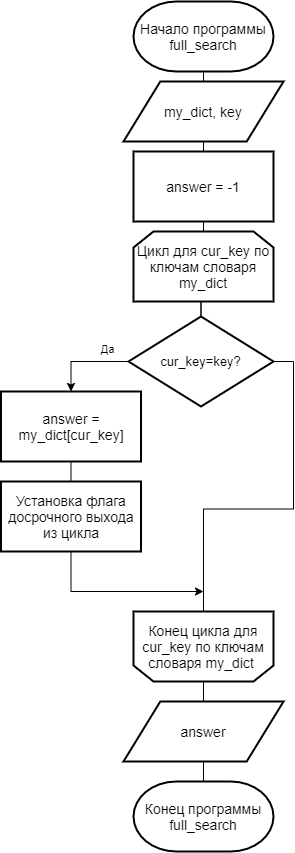
\includegraphics[scale=0.7]{inc/img/full_search.png}}
	
	\caption{Схема алгоритма полного перебора}
	
	\label{fig:full_search}
	
\end{figure}


\clearpage
\section{Схема алгоритма бинарного поиска}

На рисунке \ref{fig:binary_search} приведена схема алгоритма бинарного поиска в словаре. Предполагается, что передаваемый словарь my\_dict лексикографически упорядочен по возрастанию ключей.

\begin{figure}[h!]
	
	\centering{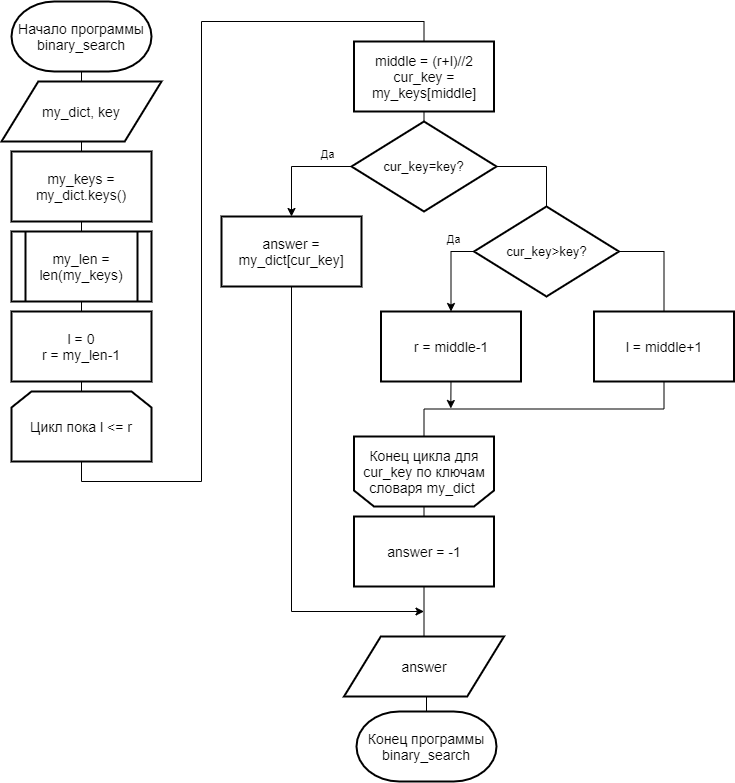
\includegraphics[scale=0.65]{inc/img/binary_search.png}}
	
	\caption{Схема алгоритма бинарного поиска}
	
	\label{fig:binary_search}
	
\end{figure}

\clearpage
\section{Схема алгоритма поиска в сегментированном словаре}

На рисунке \ref{fig:segmentate} приведена схема создания словаря, сегментированного по первым буквам ключей (все буквы английского алфавита). Такой подход к сегментации выбран, так как он является наиболее нативным для используемого словаря. Предполагается, что обращения ко всем ключам равновероятны, поэтому для ускорения поиска нужного сегмента полным перебором сегментированный словарь упорядочен по убыванию количества пар (ключ: значени) в нем. Пары внутри одого сегмента упорядочены лексикографически по возрастанию ключей для возможности реализации бинарного поиска в пределах сегмента.

\clearpage
\begin{figure}[h!]
	
	\centering{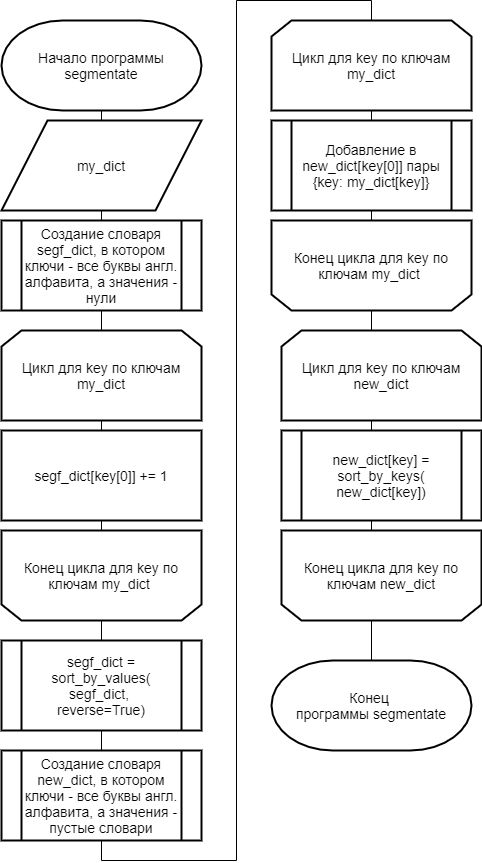
\includegraphics[scale=0.7]{inc/img/segmentate.png}}
	
	\caption{Схема создания сегментированного словаря}
	
	\label{fig:segmentate}
	
\end{figure}

На рисунке \ref{fig:segment_search} приведена схема поиска в созданном сегментированном словаре. Сначала полным перебором осуществляется поиск нужного сегмента, а затем -- бинарный поиск ключа в выбранном сегменте.

\begin{figure}[h!]
	
	\centering{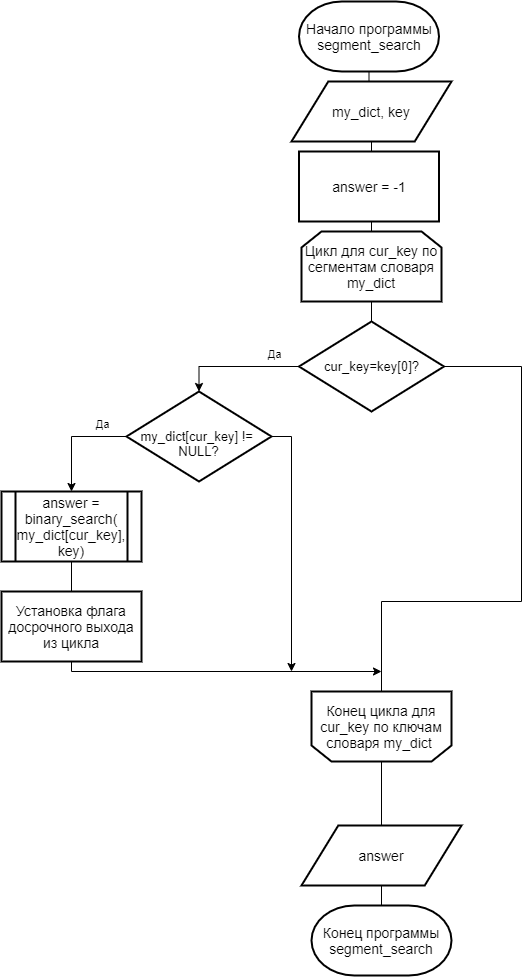
\includegraphics[scale=0.7]{inc/img/segment_search.png}}
	
	\caption{Схема поиска в сегментированном словаре}
	
	\label{fig:segment_search}
	
\end{figure}


\clearpage
\section{Вывод из конструкторской части}

Были приведены схемы разрабатываемых алгоритмов поиска в словаре: алгоритма полного перебора, алгоритма бинарного поиска и алгоритма поиска в сегментированном слолваре. 


